\documentclass[../document.tex]{subfiles}

\begin{document}
\subsection{Средства реализации}
\begin{itemize}
  \item Язык программирования - TypeScript
  \item Платформа - Node.js
\end{itemize}
\par Фронтенд:
\begin{itemize}
  \item Svelte - фронтенд-фреймворк
  \item TailwindCSS - оформление
\end{itemize}
\par Бэкенд:
\begin{itemize}
  \item SvelteKit - бэкенд-фреймворк
  \item Prisma - ORM
  \item SQLite - база данных
  \item Lucia - аутентификация
  \item Zod - валидация
  \item Vite - сборка
\end{itemize}
\subsection{Структуры данных}
\par \textbf{Пользователи}\\
Один ко многим: сессия, ключ, доски, пользователь-предмет, сообщения, логи
Один к одному: характеристики, гильдия, лидируемая гильдия,

\par \textbf{Характеристики}\\
Один ко многим: слой аватара
Один к одному: пользователь, класс

\par \textbf{Класс персонажа}\\
Один ко многим: характеристики

\par \textbf{Слой аватара}\\
Один ко многим: характеристики

\par \textbf{Задача}\\
Один к одному: приоритет, категория, доска

\par \textbf{Приоритет}\\
Один ко многим: задача

\par \textbf{Категория}\\
Один ко многим: задача

\par \textbf{Доска}\\
Один ко многим: задача
Один к одному: пользователь

\par \textbf{Тип предмета}\\
Один ко многим: предмет

\par \textbf{Предмет}\\
Один ко многим: пользователь-предмет
Один к одному: тип предмета

\par \textbf{Пользователь-предмет}\\
Один к одному: пользователь, предмет

\par \textbf{Гильдия}\\
Один ко многим: пользователи, сообщения, логи
Один к одному: лидер, босс

\par \textbf{Сообщение}\\
Один к одному: пользователь, гильдия

\par \textbf{Босс}\\
Один ко многим: гильдия

\par \textbf{Лог}\\
Один к одному: пользователь, гильдия

\par \textbf{Сессия}\\
Один к одному: пользователь

\par \textbf{Ключ}\\
Один к одному: пользователь

\subsection{Стандарт кодирования}
\par Автоматическое форматирование по стандарту Prettier
\subsection{Проект интерфейса}
\par Макет интерфейса составлен в Figma.

\par Набор цветов:

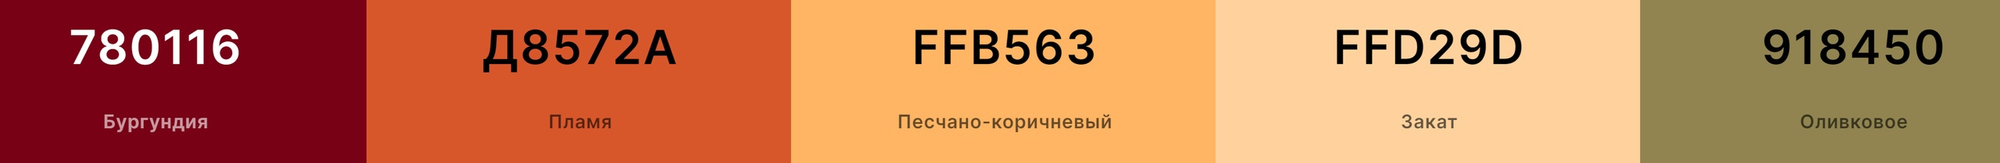
\includegraphics[width=\textwidth]{colors.png}

\par Наброски:

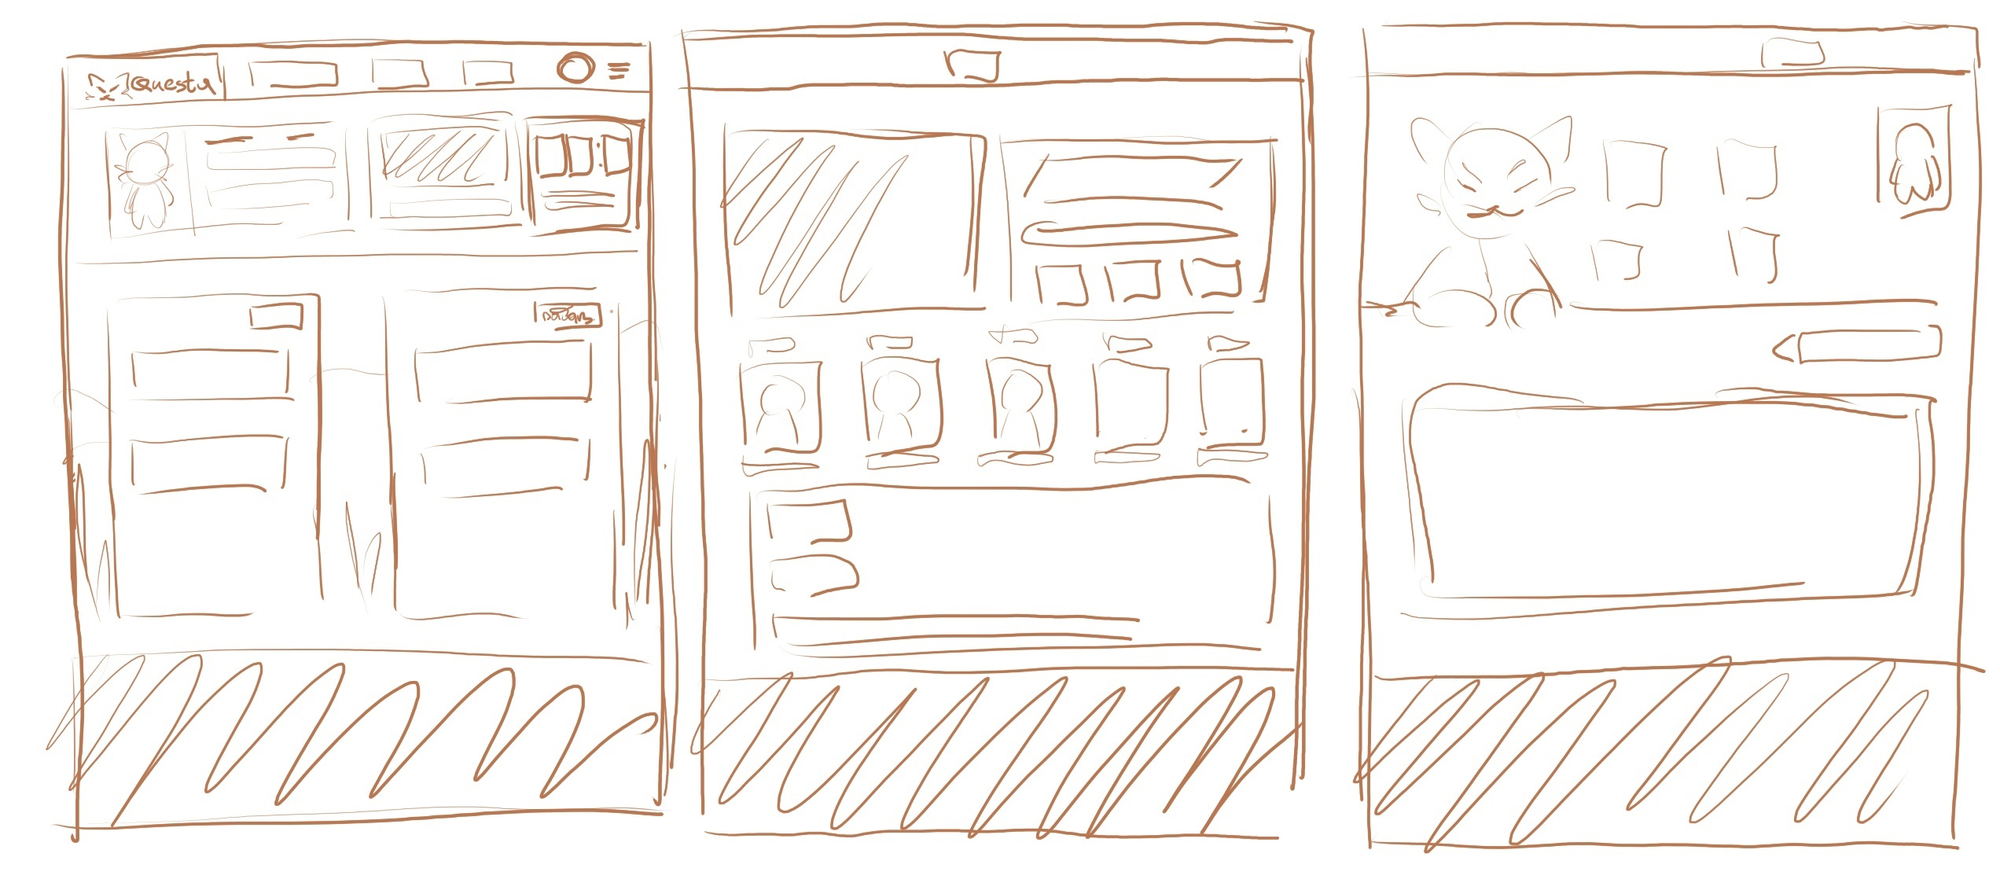
\includegraphics[width=\textwidth]{sketches1.png}

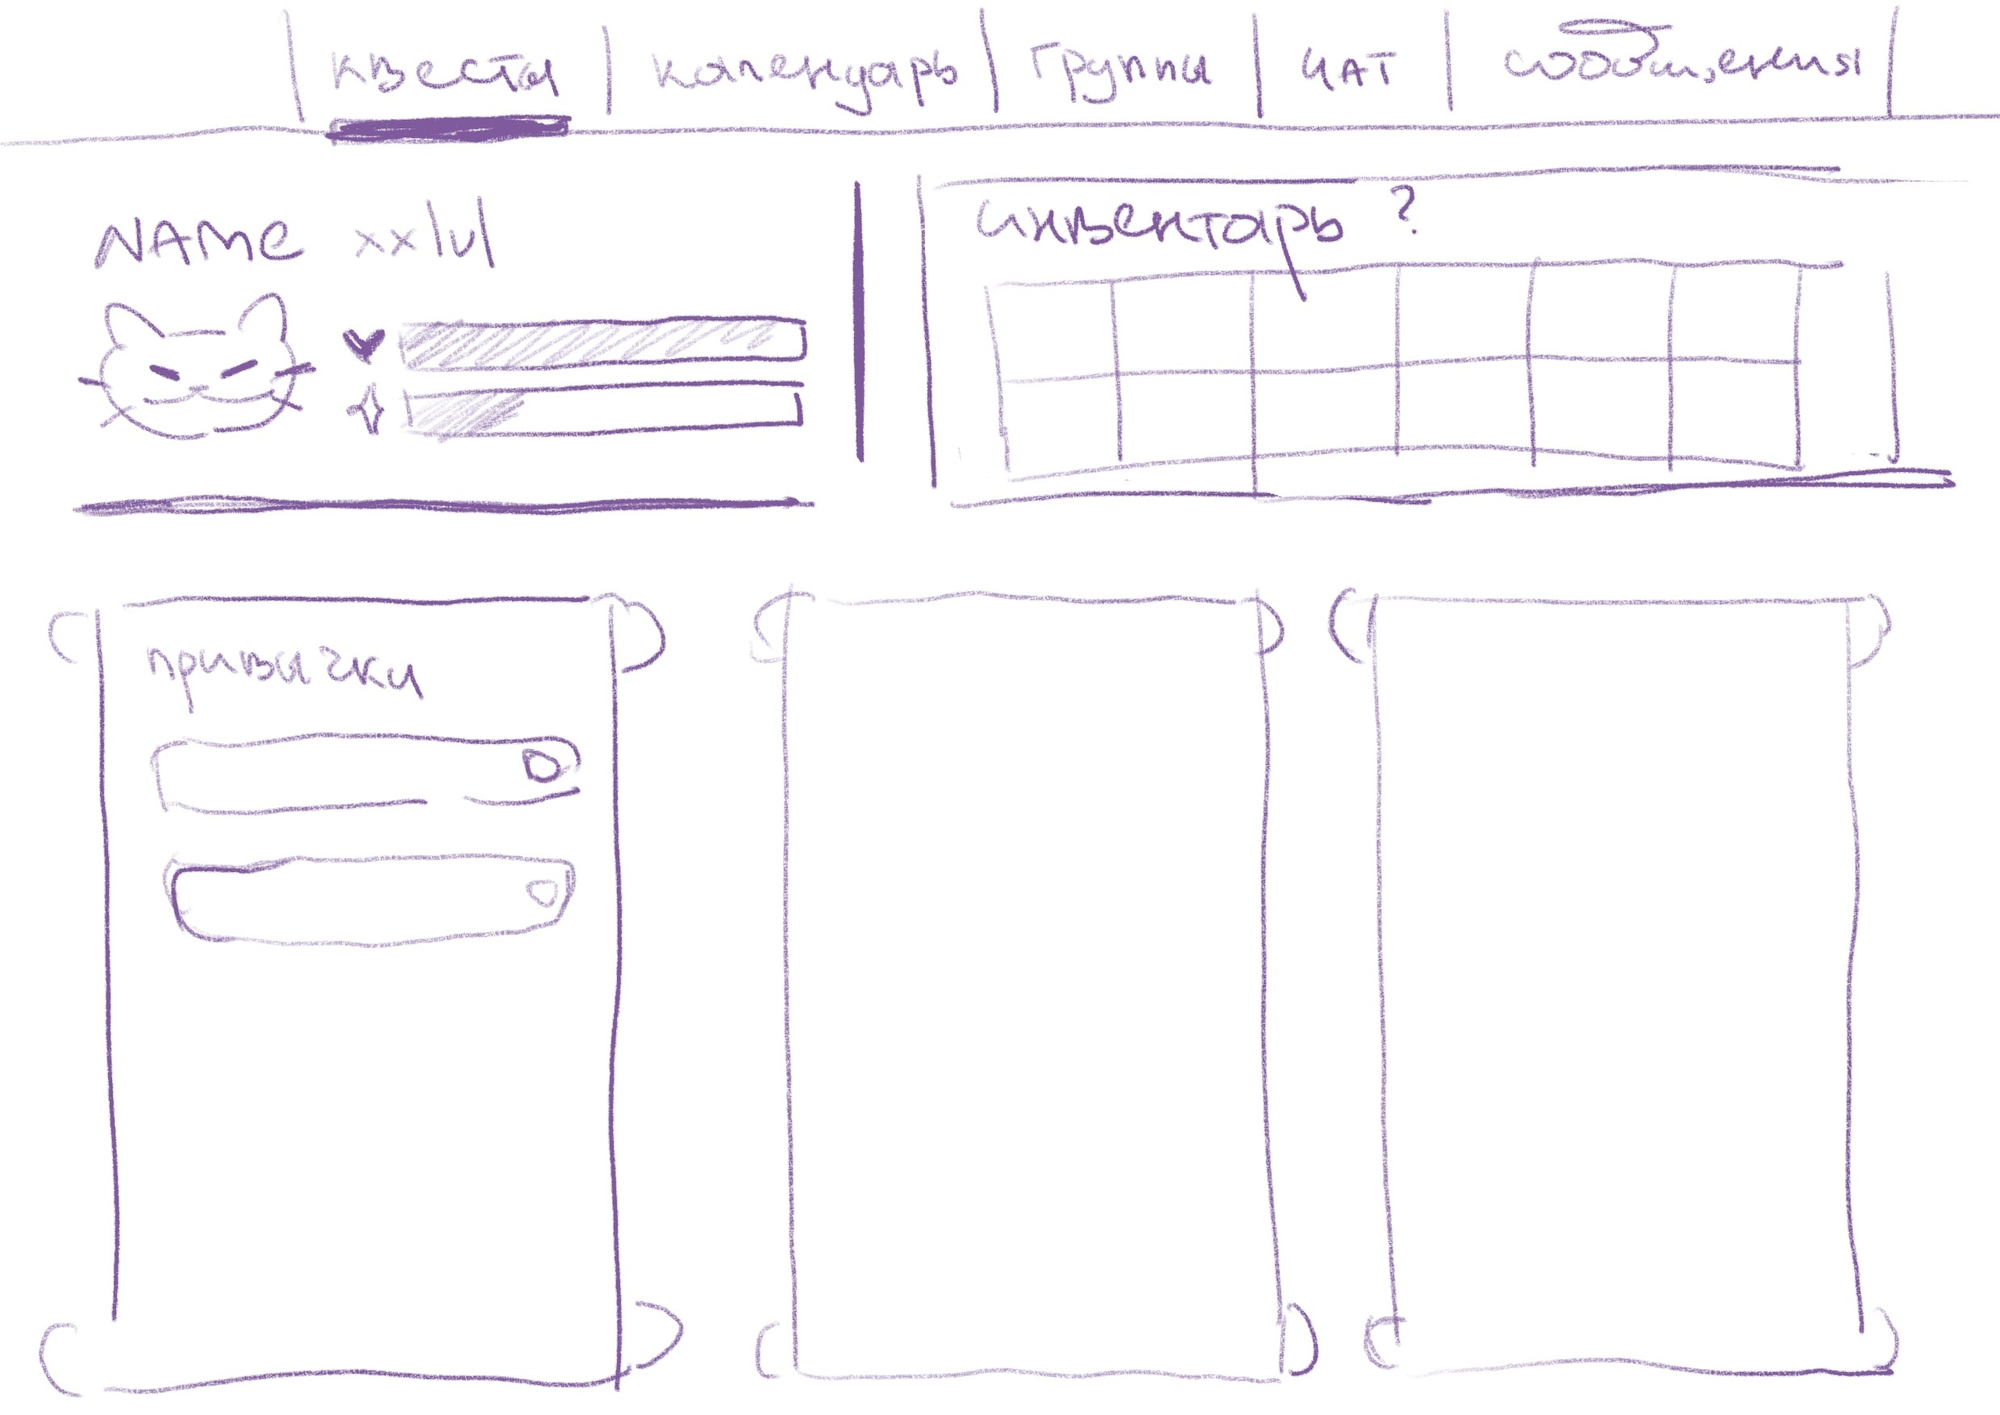
\includegraphics[width=\textwidth]{sketches2.png}

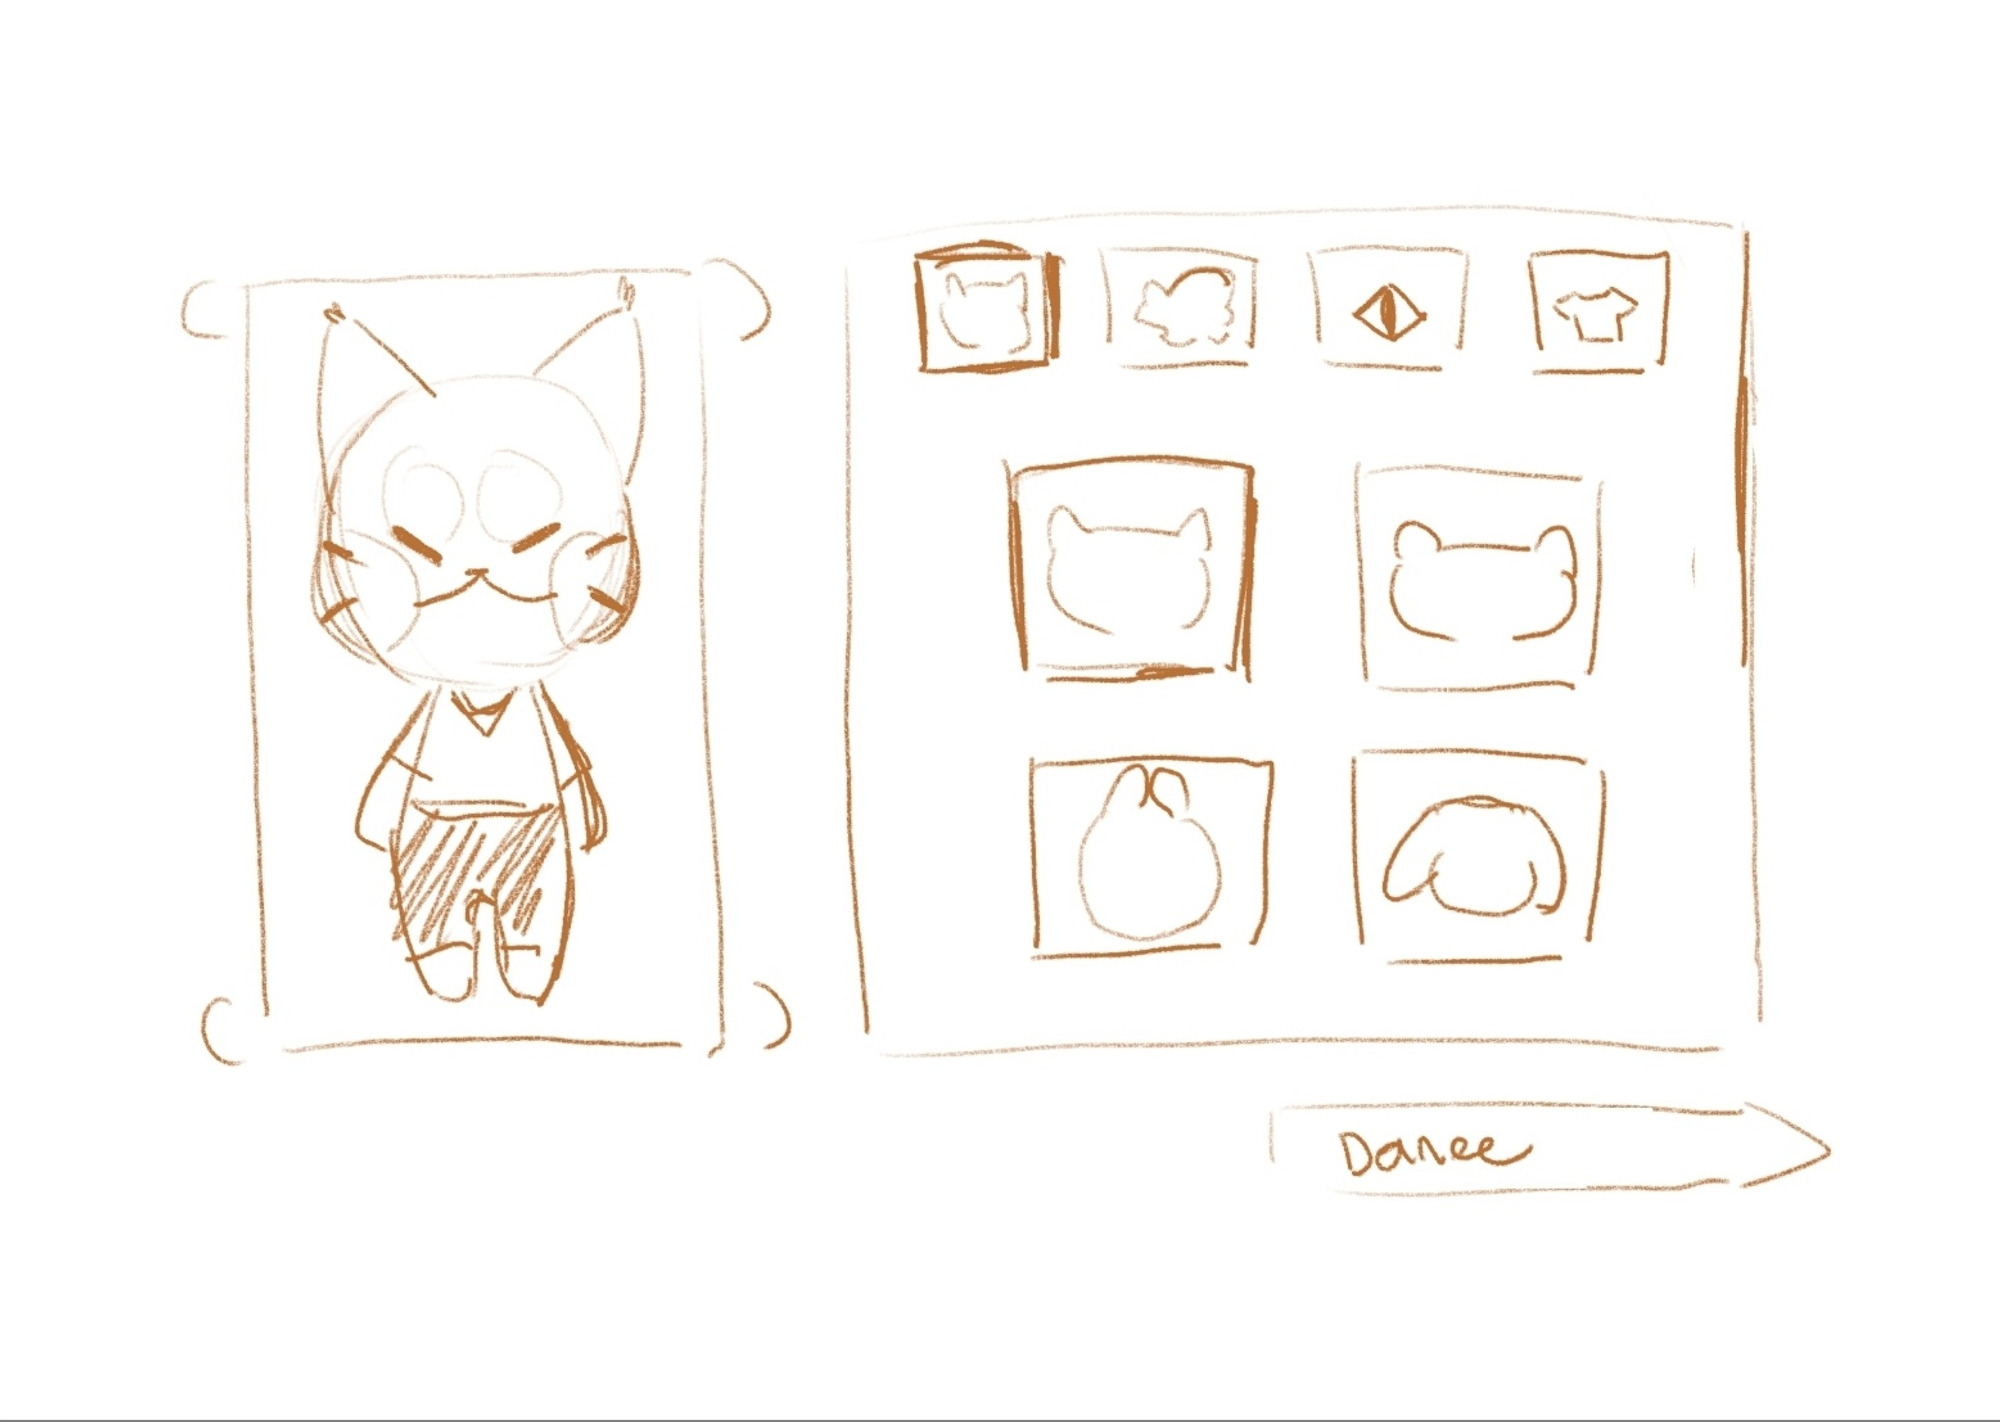
\includegraphics[width=\textwidth]{sketches3.png}

\par Снимки экрана:
\\\\
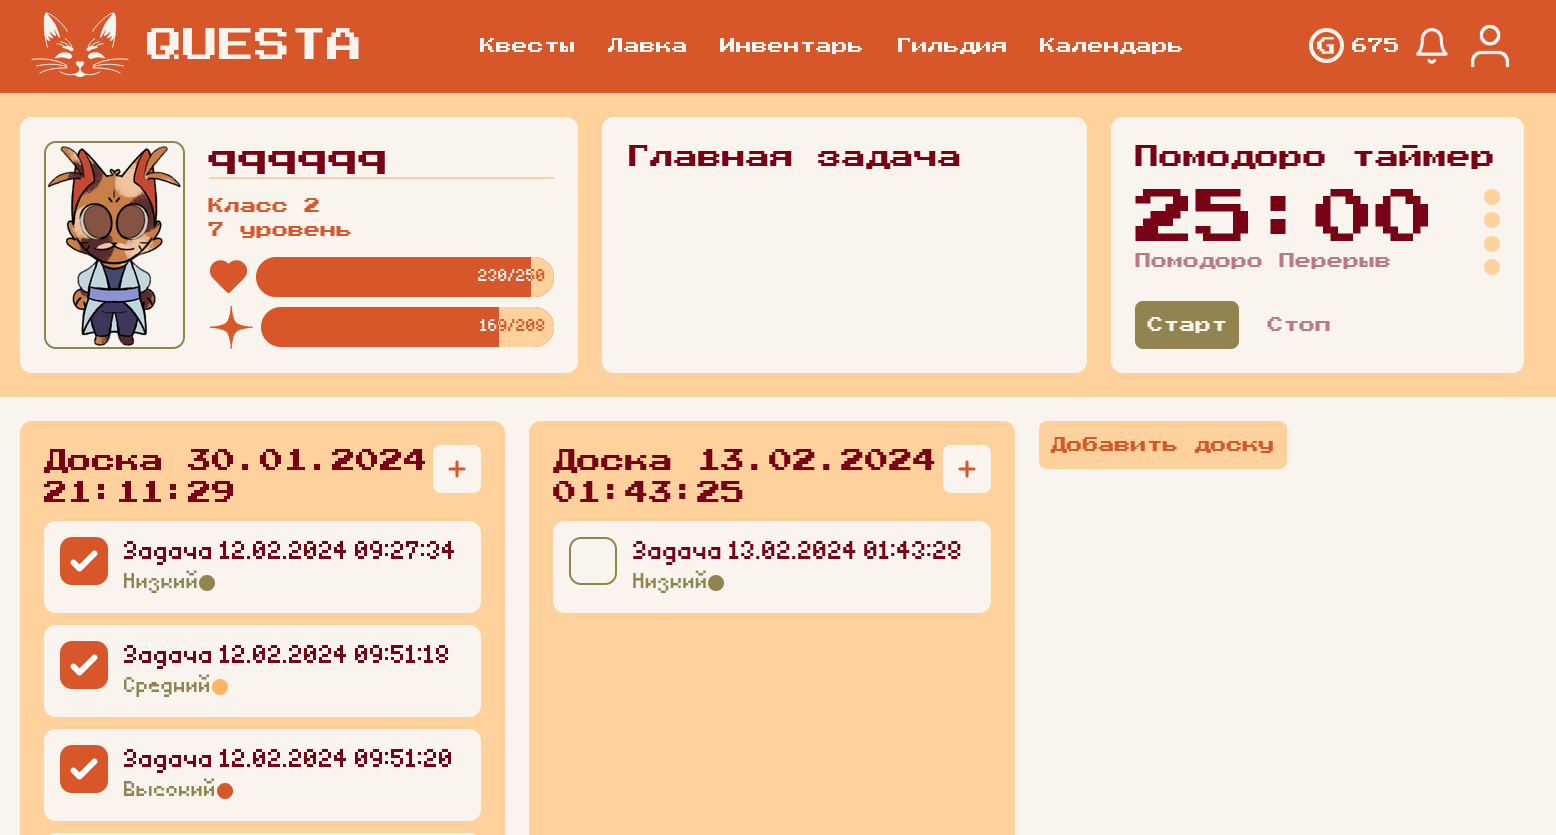
\includegraphics[width=\textwidth]{screens1.png}
\\\\
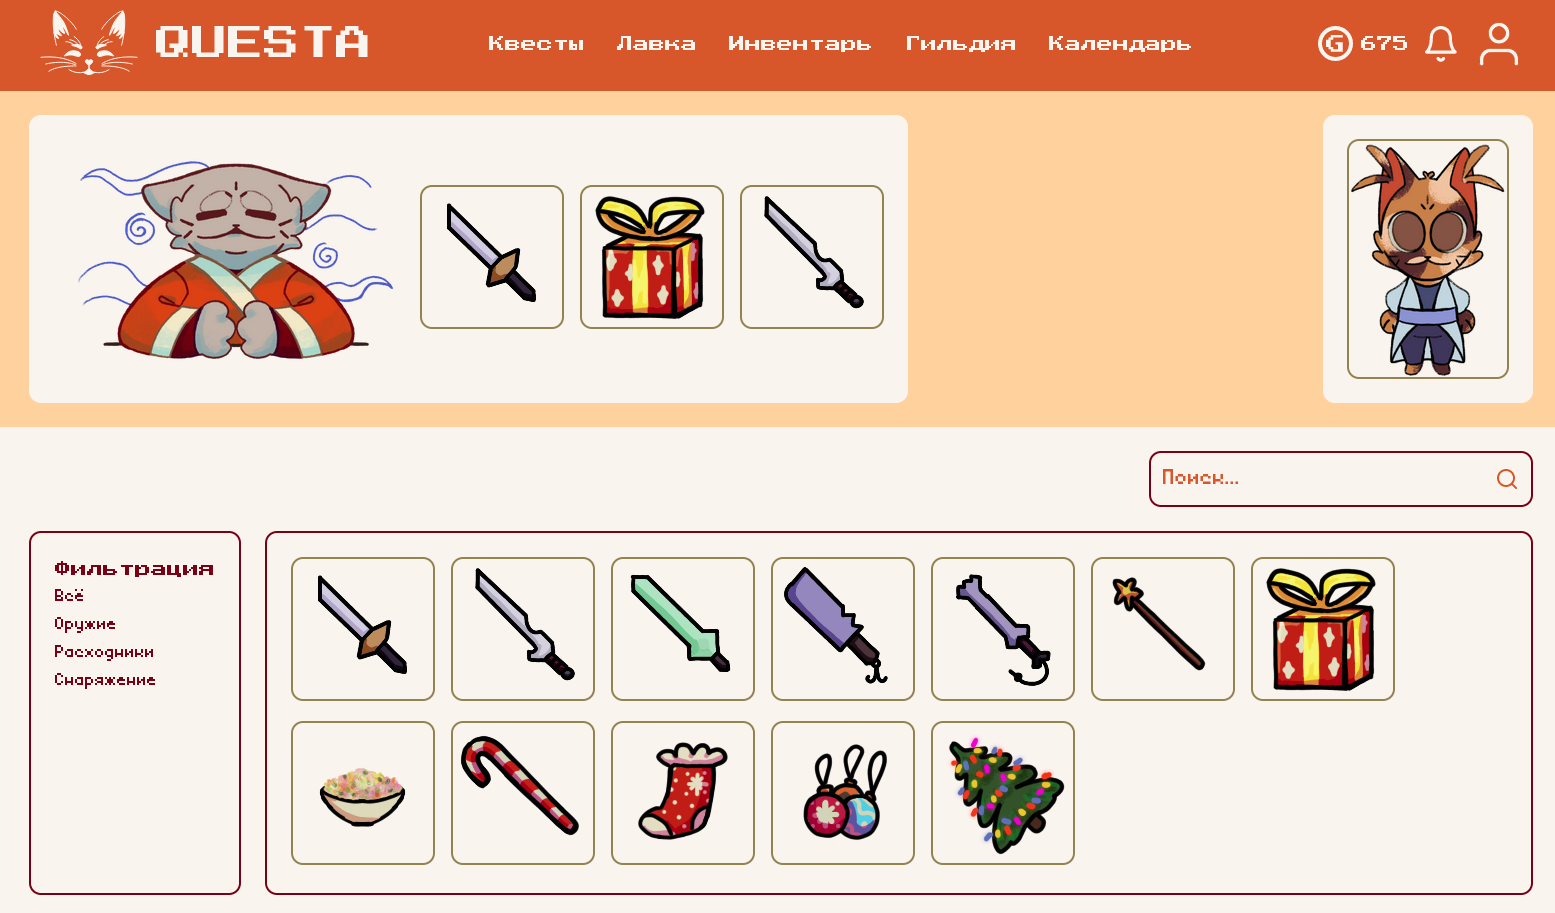
\includegraphics[width=\textwidth]{screens2.png}
\\\\
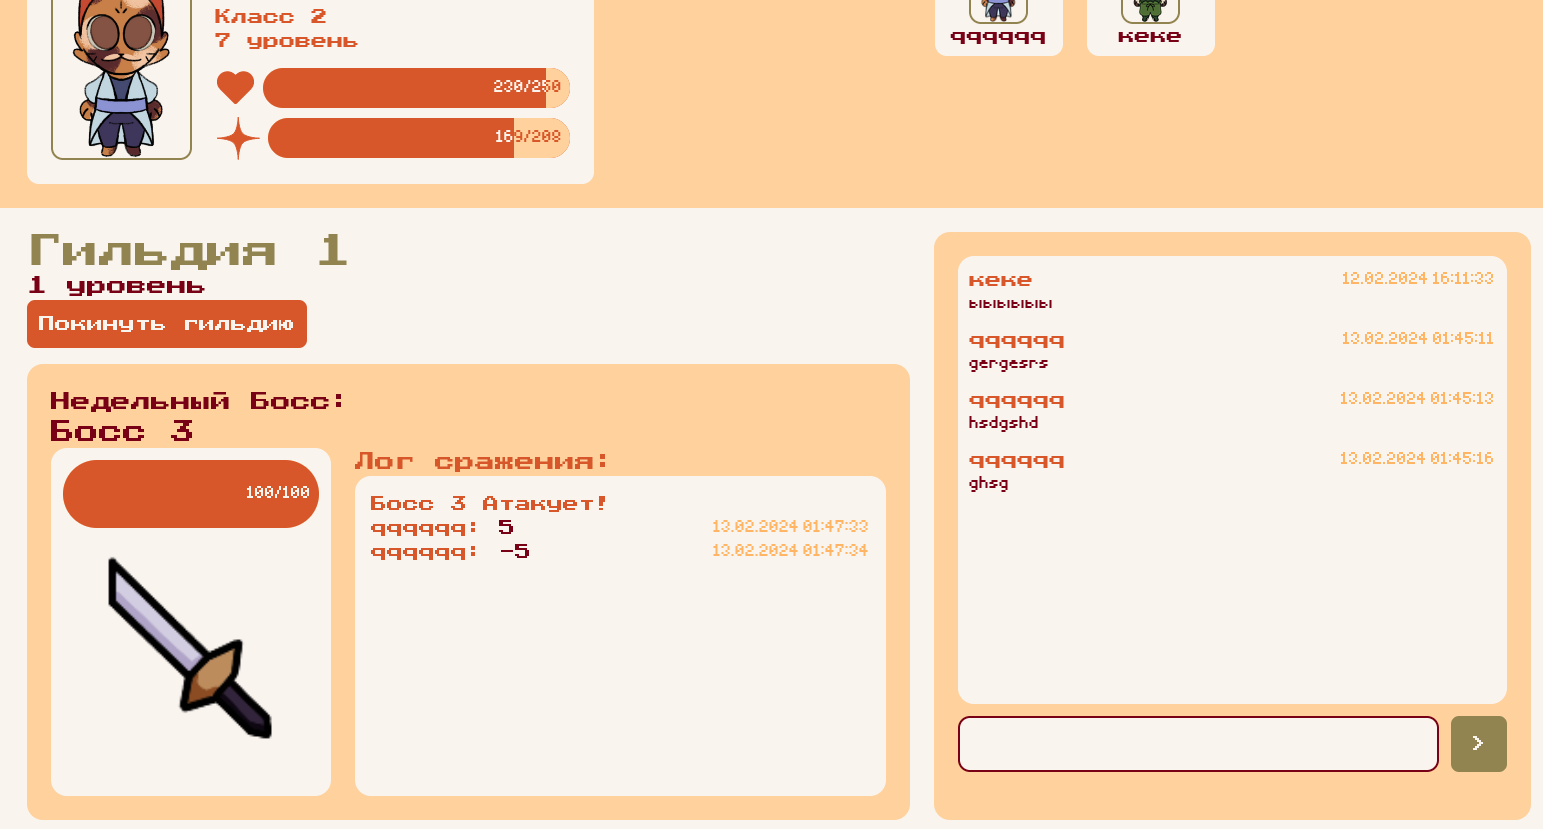
\includegraphics[width=\textwidth]{screens3.png}
\\\\
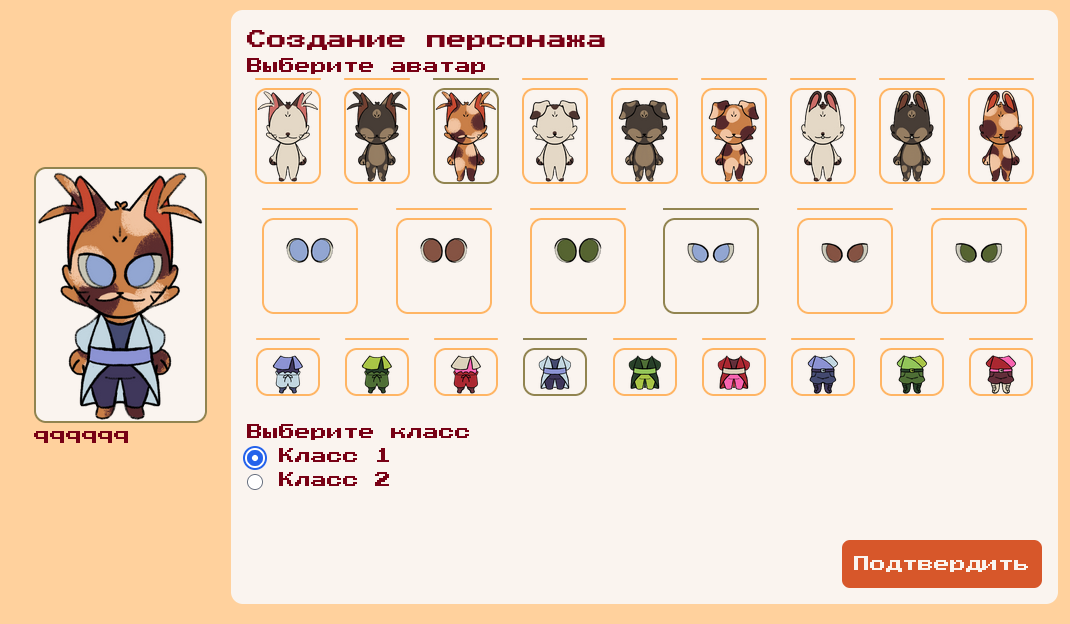
\includegraphics[width=\textwidth]{screens4.png}

\end{document}
